%%==================================================
%% chapter01.tex for BIT Master Thesis
%% modified by yang yating
%% version: 0.1
%% last update: Dec 25th, 2016
%%==================================================
\chapter{引言}
\label{chap:intro}
\section{应用背景}

模拟的调幅广播发明于二十世纪二十年代,其后虽然也有一些技术上的进步,但系统体系基本没变,存在着传输质量差、业务单一、易被干扰等比较明显的缺点,随着FM、电视和互联网等新型媒体的出现,模拟调幅广播的地位受到了重大挑战,用户规模迅速下降。因此如何利用现有频段和技术对调幅广播系统进行改造,使之能够满足时代的需要成为了各国广播运行部门和技术部门的一个重要课题。

普遍的共识是利用数字通信技术对发射系统进行数字化改造,提供新业务的同时保持模拟调幅业务的平滑过渡,仅改变发射系统的信源、编码和调制模块,尽可能利用现有的各种发射机,通常这种方案被称为数字调幅广播,或者数字AM广播。

目前虽然对于数字化广播有多种候选方案,但最成熟的并且已经成为国际标准的是所谓的DRM数字广播技术,DRM是研发该技术的Digital Radio Mondiale(法语单词)的简称,DRM数字广播于2001年成为ITU标准,2002年通过IEC审核进入实施阶段。DRM系统是经过严格试验的、技术成熟的系统,并且DRM是目前唯一的非专利的数字广播系统,各国在实施中不会遇到所谓的专利壁垒。和其他数字广播系统相比DRM数字调幅广播具有以下优点:

\begin{itemize}
	\item 大幅度降低广播功率;
	\item 显著提高信号传送的音质;
	\item 大大提高调幅频段信号传送的可靠性;
	\item 与现有模拟信号兼容,可以实现模拟数字信号同播,实现向全数字化的平滑过渡;
	\item 不改变现有频段分配,充分利用现有中短波频谱资源;
	\item 对现有发射机进行成本有限的改造,不需要增加新的发射机;
	\item 提供新的附加业务和数字传输
\end{itemize}

在系统设计上DRM采用了以下设计思想:

\begin{itemize}
	\item 采用高效的信源变码技术以满足声音质量要求的前提下有效降低码率;
	\item 采用高效的信道编码和调制技术对抗多径传输和频率选择性衰减等信道影响;
	\item 提供灵活高效的信源复用方式满足不同的业务需求。
\end{itemize}

系统的原理框图如\ref{fig:diagram}所示。

\begin{figure}
	\centering
	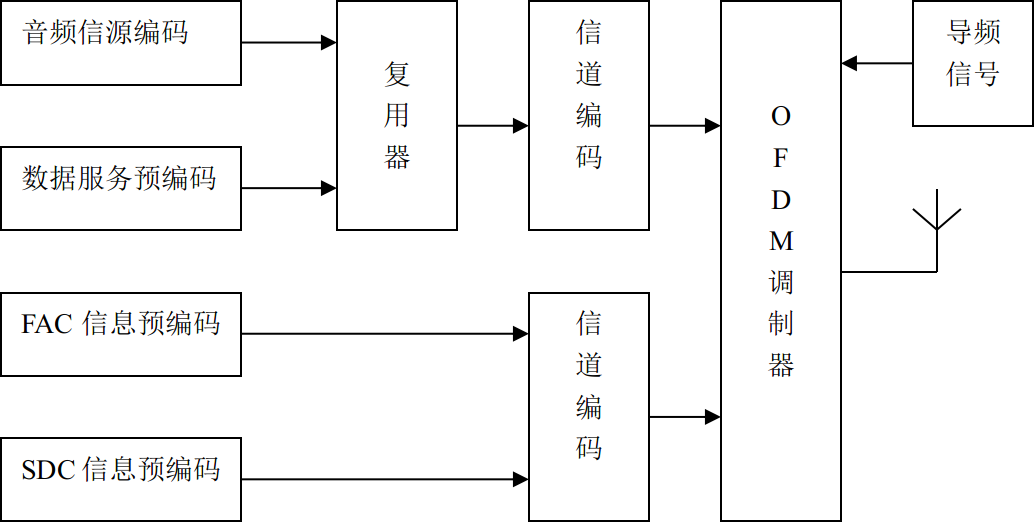
\includegraphics[width=\textwidth]{figures/figure1}
	\caption{DRM系统的原理框图}\label{fig:diagram}
\end{figure}

通常数字音频的质量由数据率决定,但高的数据率需要高的传输带宽,数据压缩技术的出现解决了数字广播中音频质量和带宽的矛盾。DRM系统中的数据压缩体现于语音编码(信源编码),其质量直接决定了声音信号的质量和系统传输所需要的频带宽度。

在DRM标准中根据不同的业务需要定义了三种不同的语音编码技术:先进音频编码AAC、码激励线性预测CELP和谐波矢量激励编码HVXC,除此之外DRM系统还采用了SBR频带复制技术,它可以在进行音频编码之前将带宽压缩为原来的1/2,解码后通过低频段波形和附加信息恢复出高频信息,在保证音质的同时可以降低30\%的数据率。DRM系统要求在比较低的数据率下达到或超过FM的音质,系统中使用的三种语音编码都源于MPEG-4的子集。MPEG-4标准的音频编码部分给出了这三种编码的算法。本文定位于研究MPEG-4音频编码中CELP编码的原理、算法验证。




\section{中低速率语音编码技术}
%\label{sec:requirements}

\subsection{多脉冲线性预测编码}
对余量信号进行深入研究后,与原始语音信号相反,余量信号中的小信号对合成语音的质量影响不大,如果对余量信号进行削波处理,即将幅度低于某一阀值的所有信号全置成零,这样,只要只要适当调整阀值就可以使余量信号的90\%的样点值为零,用余下的幅度较大的信号作为激励信号源,其合成语音并未产生明显的畸变。这就提供了一种新的编码途径。1982年,Bishnu S.Atal 和 Joel R.Remde 首先提出多脉冲线性预测编码方案。在此方案中首先规定激励脉冲序列在一定时间间隔中只能出现数目有限的非零脉冲,然后每个脉冲的位置和幅度用合成分析法和感觉加权均方误差最小的判决准则进行优化,最后用优化的脉冲序列表示余量信号作为激励信号源。这样既压缩了编码速率,有改善了合成语音的质量。这样的编码系统称为多脉冲线性预测编码(Multi-Pulse Linear Predictive Coding),简称 MPLPC。在这种编码方案中,为了求出最佳的脉冲序列,其运算量相当大,而且传送脉冲幅度和相位的信息量也比较大。由于一般多脉冲激励每10ms时间内至少需要8个非零脉冲,每个脉冲需要用幅度和相位两个参数来描述,这样非零激励脉冲传输信息为2*800个参数/秒。MPLPC 可以在9.6~16kbps范围内获得较好的合成语音质量。如果再降低编码速率,则合成语音质量将会变的很差,与多脉冲激励编码相似,但是更实用的编码方法是规则脉冲激励语音编码(Regular-Pulse Excitation Coding),简称 RPE-LPC,RPE-LPC是Ed.F.Deprettere和Peter Kroon在1985年提出的,它用一组间距一定的非零的规则脉冲代替余量信号,该脉冲的相位(即第一个非零脉冲出现的位置)和每个非零脉冲的幅度可以按照MPLPC同样的方法进行优化。在RPE-LPC的激励脉冲序列中,因为各个非零脉冲的相互位置是固定的,所以它的计算量和编码速率与MPLPC相比都要小很多。

\subsection{码激励线性预测编码}

众所周知,在速率低于1bit/采样的情况下,采用矢量量化(VQ)技术表示波形是非常有效的。1985年, Manfred R.Schroeder 和 Bishnu S.Atal 提出了用VQ码本中的码字作为激励源的线性预测编码技术。码本中每一个存储的码字矢量(简称码矢量)都可以代替余量信号作为可能的激励信号源。在编码时,对码本中的码矢量逐个进行搜索,找到与输入语音误差最小的合成语音的码矢量,只要将该码矢量的标号传送给接收端,在接收端用存储的同样的码本根据收到的标号恢复出相应的码矢量作为激励。这样的编码系统,称为码激励线性预测编码(Code Excitated Linear Predictive Coding),简称CELP,CELP在4.8-16kbps范围内可以获得质量相当高的合成语音,并且抗噪声和多次转接性能也很好。

水系聚氨酯的形态对其流动性,成膜性及加工织物的性能有重要影响,一般分为三种类型\cite{Jiang2005Size} ,如表 \ref{tab:category}所示。

\begin{table}
	\centering
	\caption{水系聚氨酯分类} \label{tab:category}
	\begin{tabular*}{0.9\textwidth}{@{\extracolsep{\fill}}cccc}
		\toprule
		类别			&水溶型		&胶体分散型		&乳液型 \\
		\midrule
		状态			&溶解$\sim$胶束	&分散		&白浊 \\
		外观			&水溶型		&胶体分散型		&乳液型 \\
		粒径$/\mu m$	&$<0.001$		&$0.001-0.1$		&$>0.1$ \\
		重均分子量	&$1000\sim 10000$	&数千$\sim 20万$ &$>5000$ \\
		\bottomrule
	\end{tabular*}
\end{table}
